\ifx\allfiles\undefined
%生成目录超链接，使用UTF8字符集
\documentclass[12pt,UTF8]{ctexart}


\usepackage{mathtools}%花括号括起的公式
\usepackage{enumerate}%列表
\usepackage{graphicx}%表格
\usepackage[table]{xcolor}%彩色表格
\usepackage{booktabs}%调整表格行高


\renewcommand\tabcolsep{50pt}
\renewcommand\arraystretch{2}

%文本框
\usepackage{tcolorbox}
\tcbuselibrary{skins,vignette,raster,listings,listingsutf8,theorems, breakable,magazine,fitting}

%页面设置
\usepackage{geometry}%设置页面
\usepackage{setspace}%设置局部行距

\usepackage{ctex}
\usepackage{CJK}

%图像处理
\usepackage{graphicx}
\usepackage{float}%允许浮动
\usepackage{caption}%设置标题
\usepackage{graphicx, subfig}

%附录
\usepackage[toc,page]{appendix}

%导言区
\title{中小微企业的信贷决策}

%不要页眉
\pagestyle{plain}
\bibliographystyle{plain}

\geometry{a4paper}%将纸张设置为A4大小

%修改文档结构层次的名称
\usepackage{titlesec}%chapter1修改为一
\titleformat{\part}{\centering\Huge\bfseries}{\thepart}{1em}{}
\renewcommand\thepart{\chinese{part}}

%subsubsubsection的使用
%\usepackage{titlesec}
%\titleclass{\subsubsubsection}{straight}[\subsection]
%
%\newcounter{subsubsubsection}[subsubsection]
%\renewcommand\thesubsubsubsection{\thesubsubsection.\arabic{subsubsubsection}}
%\renewcommand\theparagraph{\thesubsubsubsection.\arabic{paragraph}}
%
%\titleformat{\subsubsubsection}
%{\normalfont\normalsize\bfseries}{\thesubsubsubsection}{1em}{}
%\titlespacing*{\subsubsubsection}
%{0pt}{3.25ex plus 1ex minus .2ex}{1.5ex plus .2ex}
%
%\makeatletter
%\renewcommand\paragraph{\@startsection{paragraph}{5}{\z@}%
%	{3.25ex \@plus1ex \@minus.2ex}%
%	{-1em}%
%	{\normalfont\normalsize\bfseries}}
%\renewcommand\subparagraph{\@startsection{subparagraph}{6}{\parindent}%
%	{3.25ex \@plus1ex \@minus .2ex}%
%	{-1em}%
%	{\normalfont\normalsize\bfseries}}
%\def\toclevel@subsubsubsection{4}
%\def\toclevel@paragraph{5}
%\def\toclevel@paragraph{6}
%\def\l@subsubsubsection{\@dottedtocline{4}{7em}{4em}}
%\def\l@paragraph{\@dottedtocline{5}{10em}{5em}}
%\def\l@subparagraph{\@dottedtocline{6}{14em}{6em}}
%\makeatother
%
%\setcounter{secnumdepth}{4}

\begin{document}
\else
\fi
%分文件开始


\section{问题二模型的建立和求解}
\subsection{构建进行信誉评级的决策树模型}
\subsubsection{决策树理论简介}

下面我们简要介绍一下决策树理论\cite{ref2}。所谓决策树，顾名思义，是一种为了解决分类问题依托策略抉择而建立起来的树。通过采用树形结构，使用层层推理来实现最终的分类。通常决策树包含下面三种主要元素，一是根节点，其包含样本的全集；二是内部节点，其对应特征属性的测试；三是叶节点，其代表决策的结果。

\begin{figure}[htbp]
	\centering
	\begin{minipage}[t]{0.49\linewidth}
		\centering
		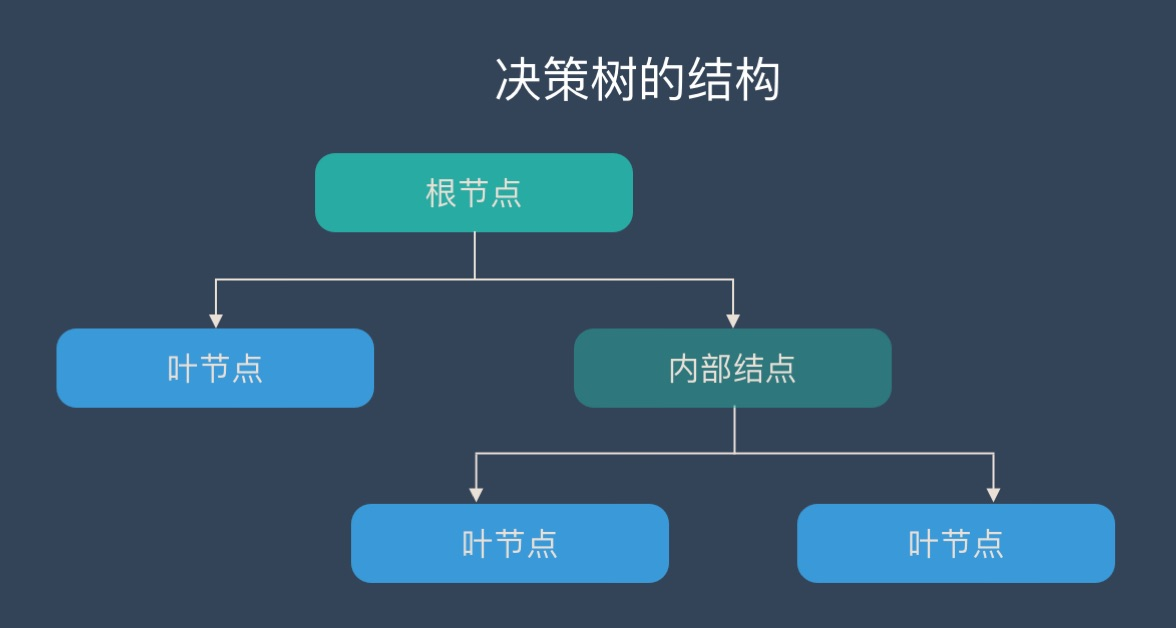
\includegraphics[height=0.15\textheight,width=0.75\linewidth]{figure/q2DecisionMakingTree1}%宽度，源文件相对位置
		\caption{决策树的结构}%图片下方的标题
	\end{minipage}
	\begin{minipage}[t]{0.49\textwidth}
		\centering
		
\includegraphics[height=0.15\textheight,width=0.75\linewidth]{figure/q2DecisionMakingTree2}%宽度，源文件相对位置
		\caption{决策树学习三步骤}%图片下方的标题
	\end{minipage}
\end{figure}

在运用决策树理论\cite{ref2}的过程中，首先需根据信息增益的原则，进行特征选择，从而筛选出跟分类结果相关性较高的特征。接着从根节点触发，对节点计算所有特征的信息增益，选择信息增益最大的特征作为节点特征，并根据该特征的不同取值建立子节点。之后对每个子节点使用相同的方式生成新的子节点，直到信息增益很小或者没有特征可以选择为止，进而生成决策树。最后对已生成好的决策树进行剪枝，通过主动去掉部分分支来降低过拟合的风险，得到最终分类结果。

\subsubsection{据已有信誉评级训练决策树模型}

在建立决策树模型过程中，我们通过MPai数据科学平台来训练决策树。所谓MPai数据科学平台是一款基础性数据分析软件，以低门槛、一站式、规范化、高效率为主要特征，使我们能够快速掌握数据分析。在MPai平台，我们首先创建一个工程来存放数据与分析结果，接着我们将数据导入相应文件夹，之后我们配置决策树模型，根据已有信誉评级设置如下表所示的相应工程参数，最后便可在分析结果页查看最终训练结果，快速得出最拟合数据的模型特征概要。


根据如上表格设置相应参数后进行求解，所得到的结果如下：

\begin{figure}[H]
	\centering
	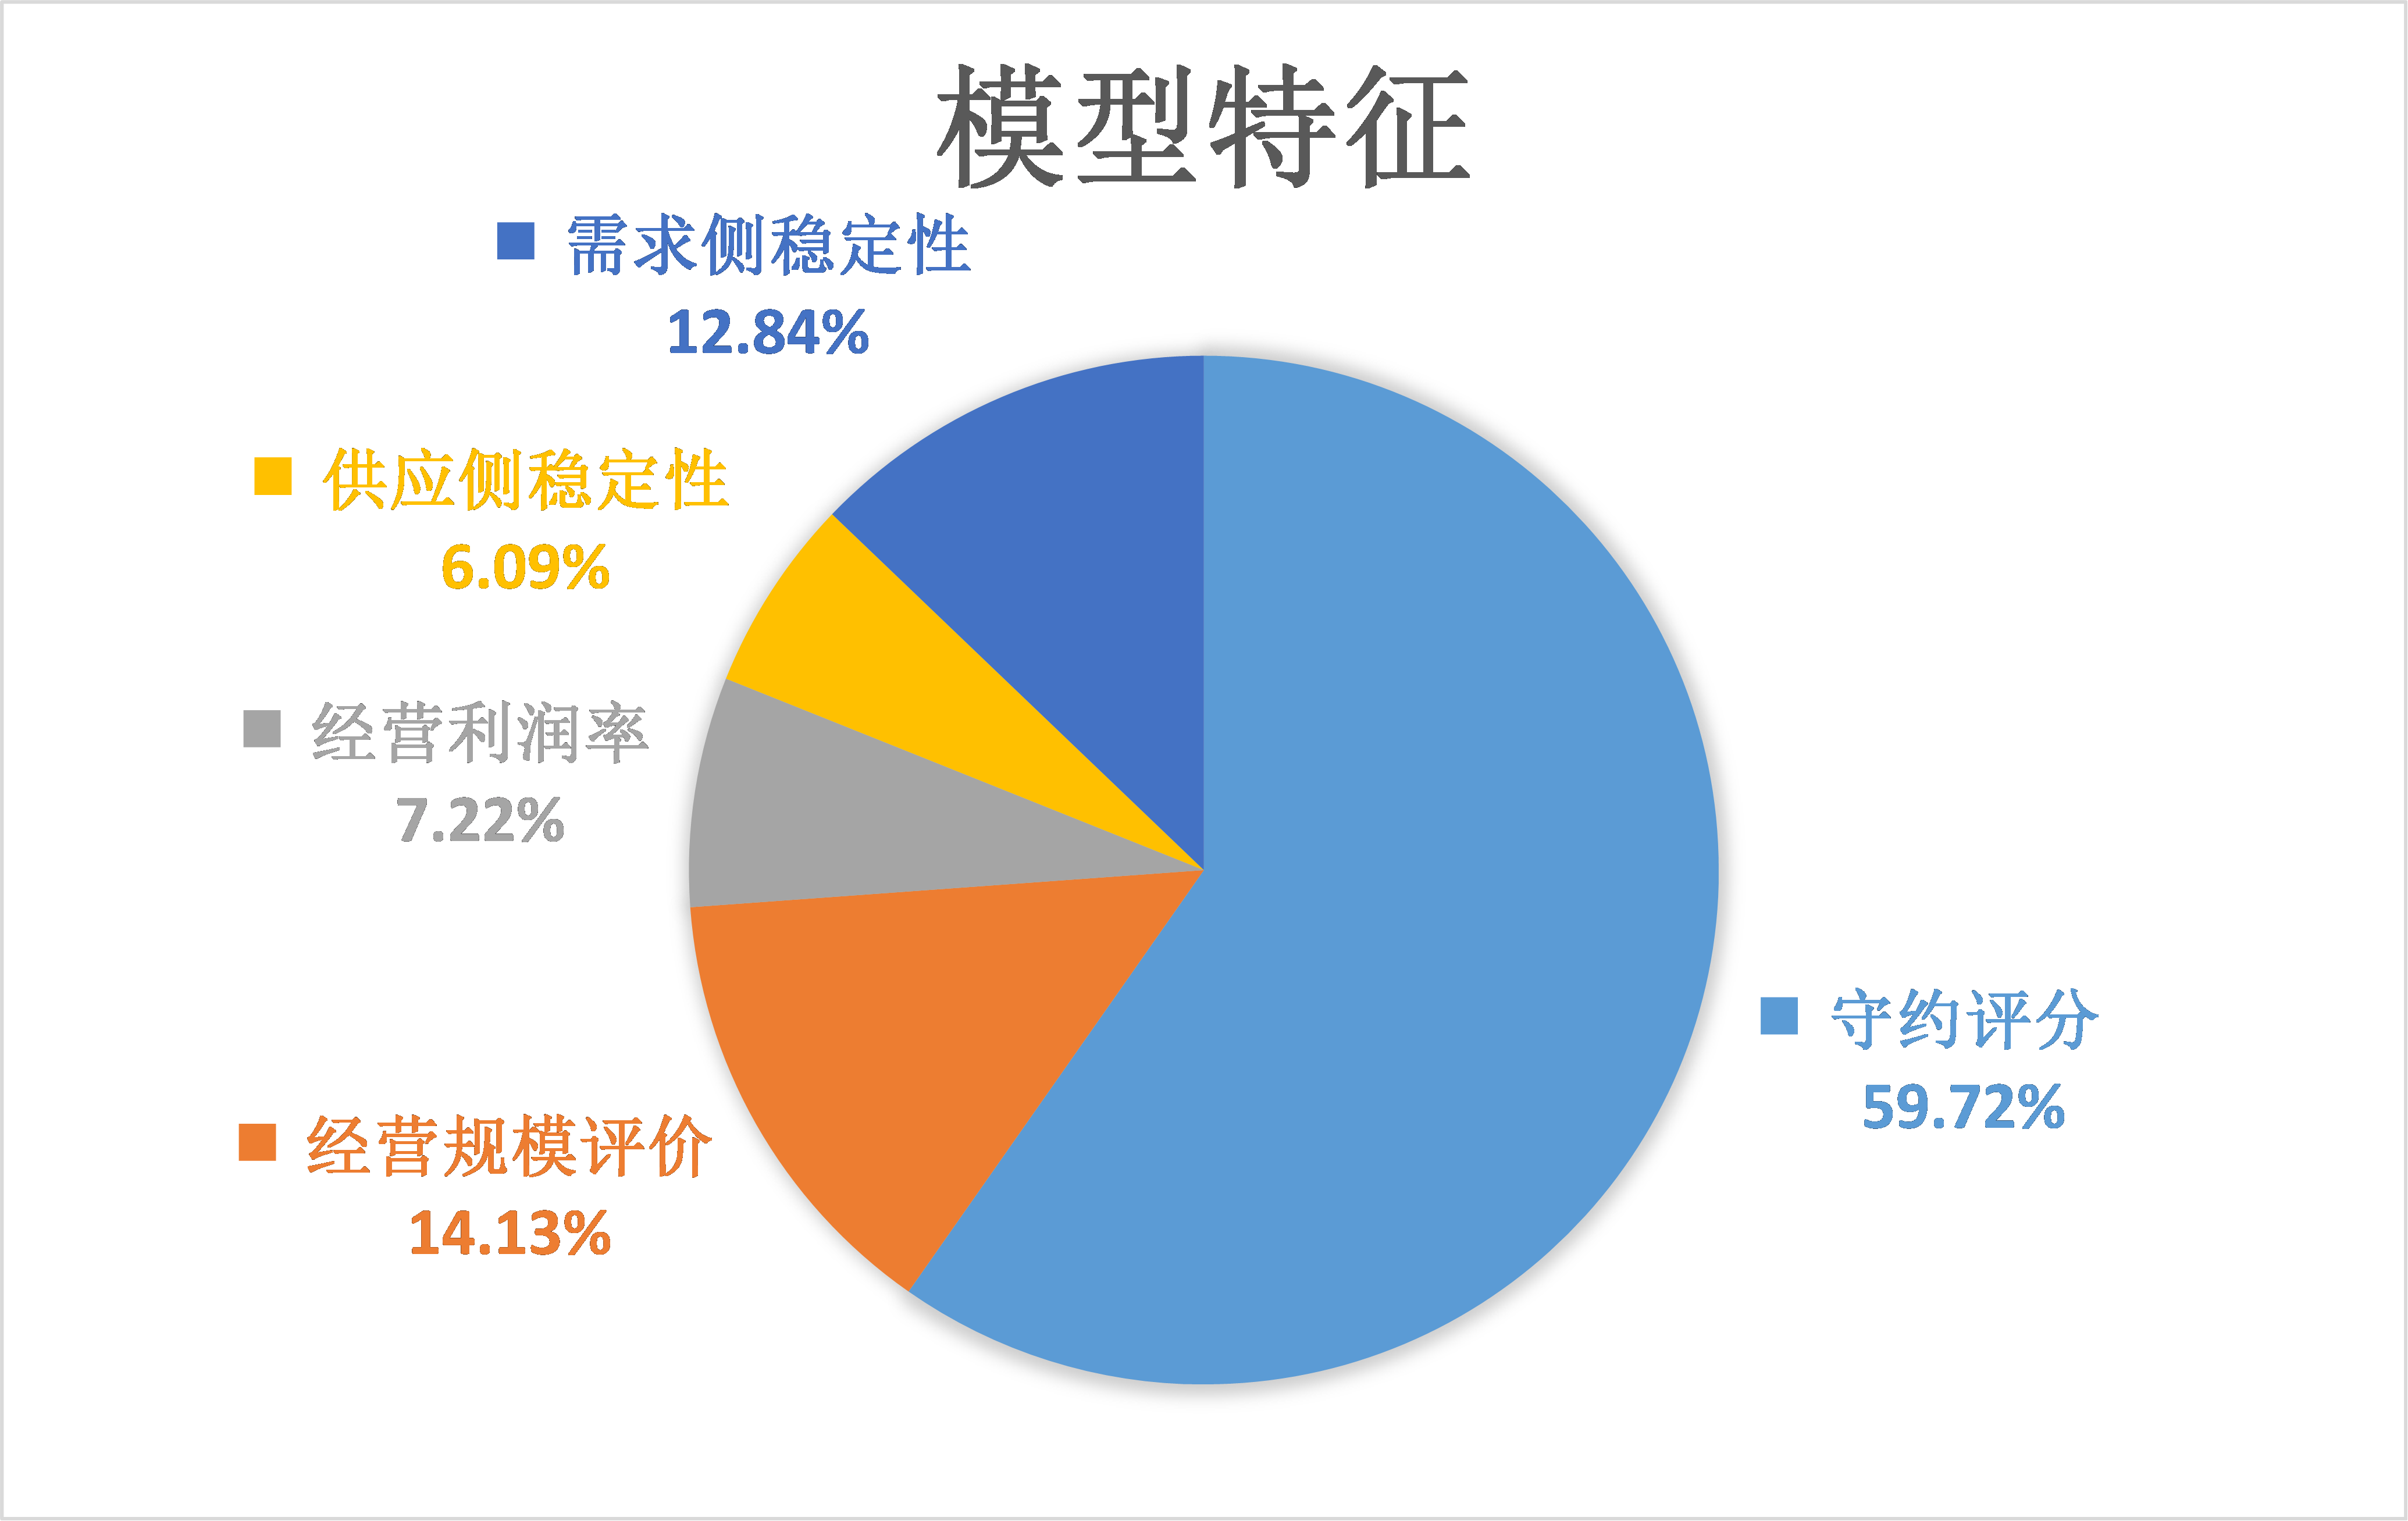
\includegraphics[width=0.75\linewidth]{figure/q2ModelAnalysis}%宽度，源文件相对位置
	\caption{模型特征}%图片下方的标题
	\label{fig:q2ModelAnalysis}%图片引用时所需标签
\end{figure}

\subsubsection{决策树模型的评价}

在模型建立方面，我们通过在MPai数据科学平台上训练决策树，得到如下评估结果，评价指标包括$ MSE $，$ RMSE $，$ MAE $，$ R^{2} $，$ MAPE $\cite{ref2}。

$ MSE $即均方误差，范围[0,+∞) ，当预测值与真实值完全吻合时等于0，即完美模型；误差越大，该值越大。

$ RMSE $即均方根误差，范围[0,+∞)，当预测值与真实值完全吻合时等于0，即完美模型；误差越大，该值越大。

$ MAE $即平均绝对误差，范围[0,+∞)，当预测值与真实值完全吻合时等于0，即完美模型；误差越大，该值越大。

$ R^{2} $即相关系数，范围[0,1]，是一个评价拟合好坏的指标。一般来说，$ R^{2} $越大，表示模型拟合效果越好。

$ MAPE $即平均绝对百分比误差，范围[0,+∞)，等于$0\%$表示完美模型，大于  $100\%$则表示劣质模型。

由我们得到的评估结果如下表所示，说明我们的模型建立的预测值与真实值的误差很小，是几乎吻合的。

\begin{center}
	\begin{table}[H]  %table 里面也可以嵌套tabular,只有tabular是不能加标题的
		\centering
		\caption{测试数据评估结果}  %表格标题
		\resizebox{250pt}{75pt}{
			\begin{tabular}{cr}
				\hline
				评价指标  & 评价结果 \\
				\hline
				$ MSE $   & 60.6317  \\
				$ RMSE $  & 7.7866   \\
				$ MAE $   & 34.6613  \\
				$ R^{2} $ & 0.3807   \\
				$ MAPE $  & 55.9964  \\
				\hline
			\end{tabular}}
	\end{table}
\end{center}


\subsection{量化分析信贷风险}
\subsubsection{用决策树模型进行信誉评级}

利用MPai数据科学平台配置好决策树模型后，将前述处理得到的302家企业的各项指标数据导入创建好的工程中，并在结果页查看最终预测结果。下面展示了利用决策树模型处理得到的前10个数据的预测结果：

\begin{center}
	\begin{table}[H]  %table 里面也可以嵌套tabular,只有tabular是不能加标题的
		\centering
		\caption{决策树模型各指标前10个数据展示}  %表格标题
		\resizebox{300pt}{75pt}{
			\begin{tabular}{ccrrrr}
				\hline
				预测结果Y & 守约评分 & 经营规模评分 & 经营利润率 & 供应侧稳定性 & 需求供应侧稳定性 \\
				\hline
				4.00      & 1        & 0.7881       & -0.0652    & 0.8411       & 0.8183           \\
				4.00      & 1        & 1.0000       & -0.0063    & 0.8406       & 0.8389           \\
				2.00      & 1        & 0.5532       & 3.5657     & 0.9550       & 0.8127           \\
				4.00      & 1        & 0.6926       & 29.9004    & 0.9793       & 0.9687           \\
				2.00      & 1        & 0.2575       & 13.4326    & 0.9634       & 0.9251           \\
				4.00      & 1        & 0.3451       & 1.7936     & 0.9285       & 0.8759           \\
				3.00      & 1        & 0.1169       & 0.4182     & 0.9496       & 0.9407           \\
				3.50      & 1        & 0.2221       & 0.6050     & 0.8858       & 0.9158           \\
				3.67      & 1        & 0.2160       & 1.6892     & 0.9750       & 0.9182           \\
				3.67      & 1        & 0.1207       & 1.7742     & 0.9696       & 0.8059           \\
				\hline
			\end{tabular}}
	\end{table}
\end{center}


\subsubsection{用层次分析法量化分析信贷风险}

首先，构建与问题一相类似的层次结构图\cite{ref1}，将决策目标，即目标层，定为量化分析企业信贷风险；决策准则，即准则层，定为守约评分、经营规模、盈利能力、供应侧稳定性、需求侧稳定性、信誉评级六个因素；决策对象，即方案层，定为302家公司的信贷能力。

其次，采用相对尺度法，通过比较六个因素两两之间的相对重要程度，构造出量化分析企业信贷风险，即目标层，与六个因素，即准则层，之间的成对比较矩阵。

然后，我们在MATLAB中调用预先编写好的函数\verb|AHP()|，该函数的代码可以在附录中找到。接着便可得到对应的权重向量$ W $、最大特征值$ L_{max} $、一致性指标$ CI $以及一致性比率$ CR $。利用$ CI $与$ CR $，对所得出的权重向量，进行一致性检验，判断出该权重向量可作为最终的决策依据。

最后运用该权重向量，分别计算出302家企业各自的信贷能力，以此来分析其信贷风险。

\begin{figure}[H]
	\centering
	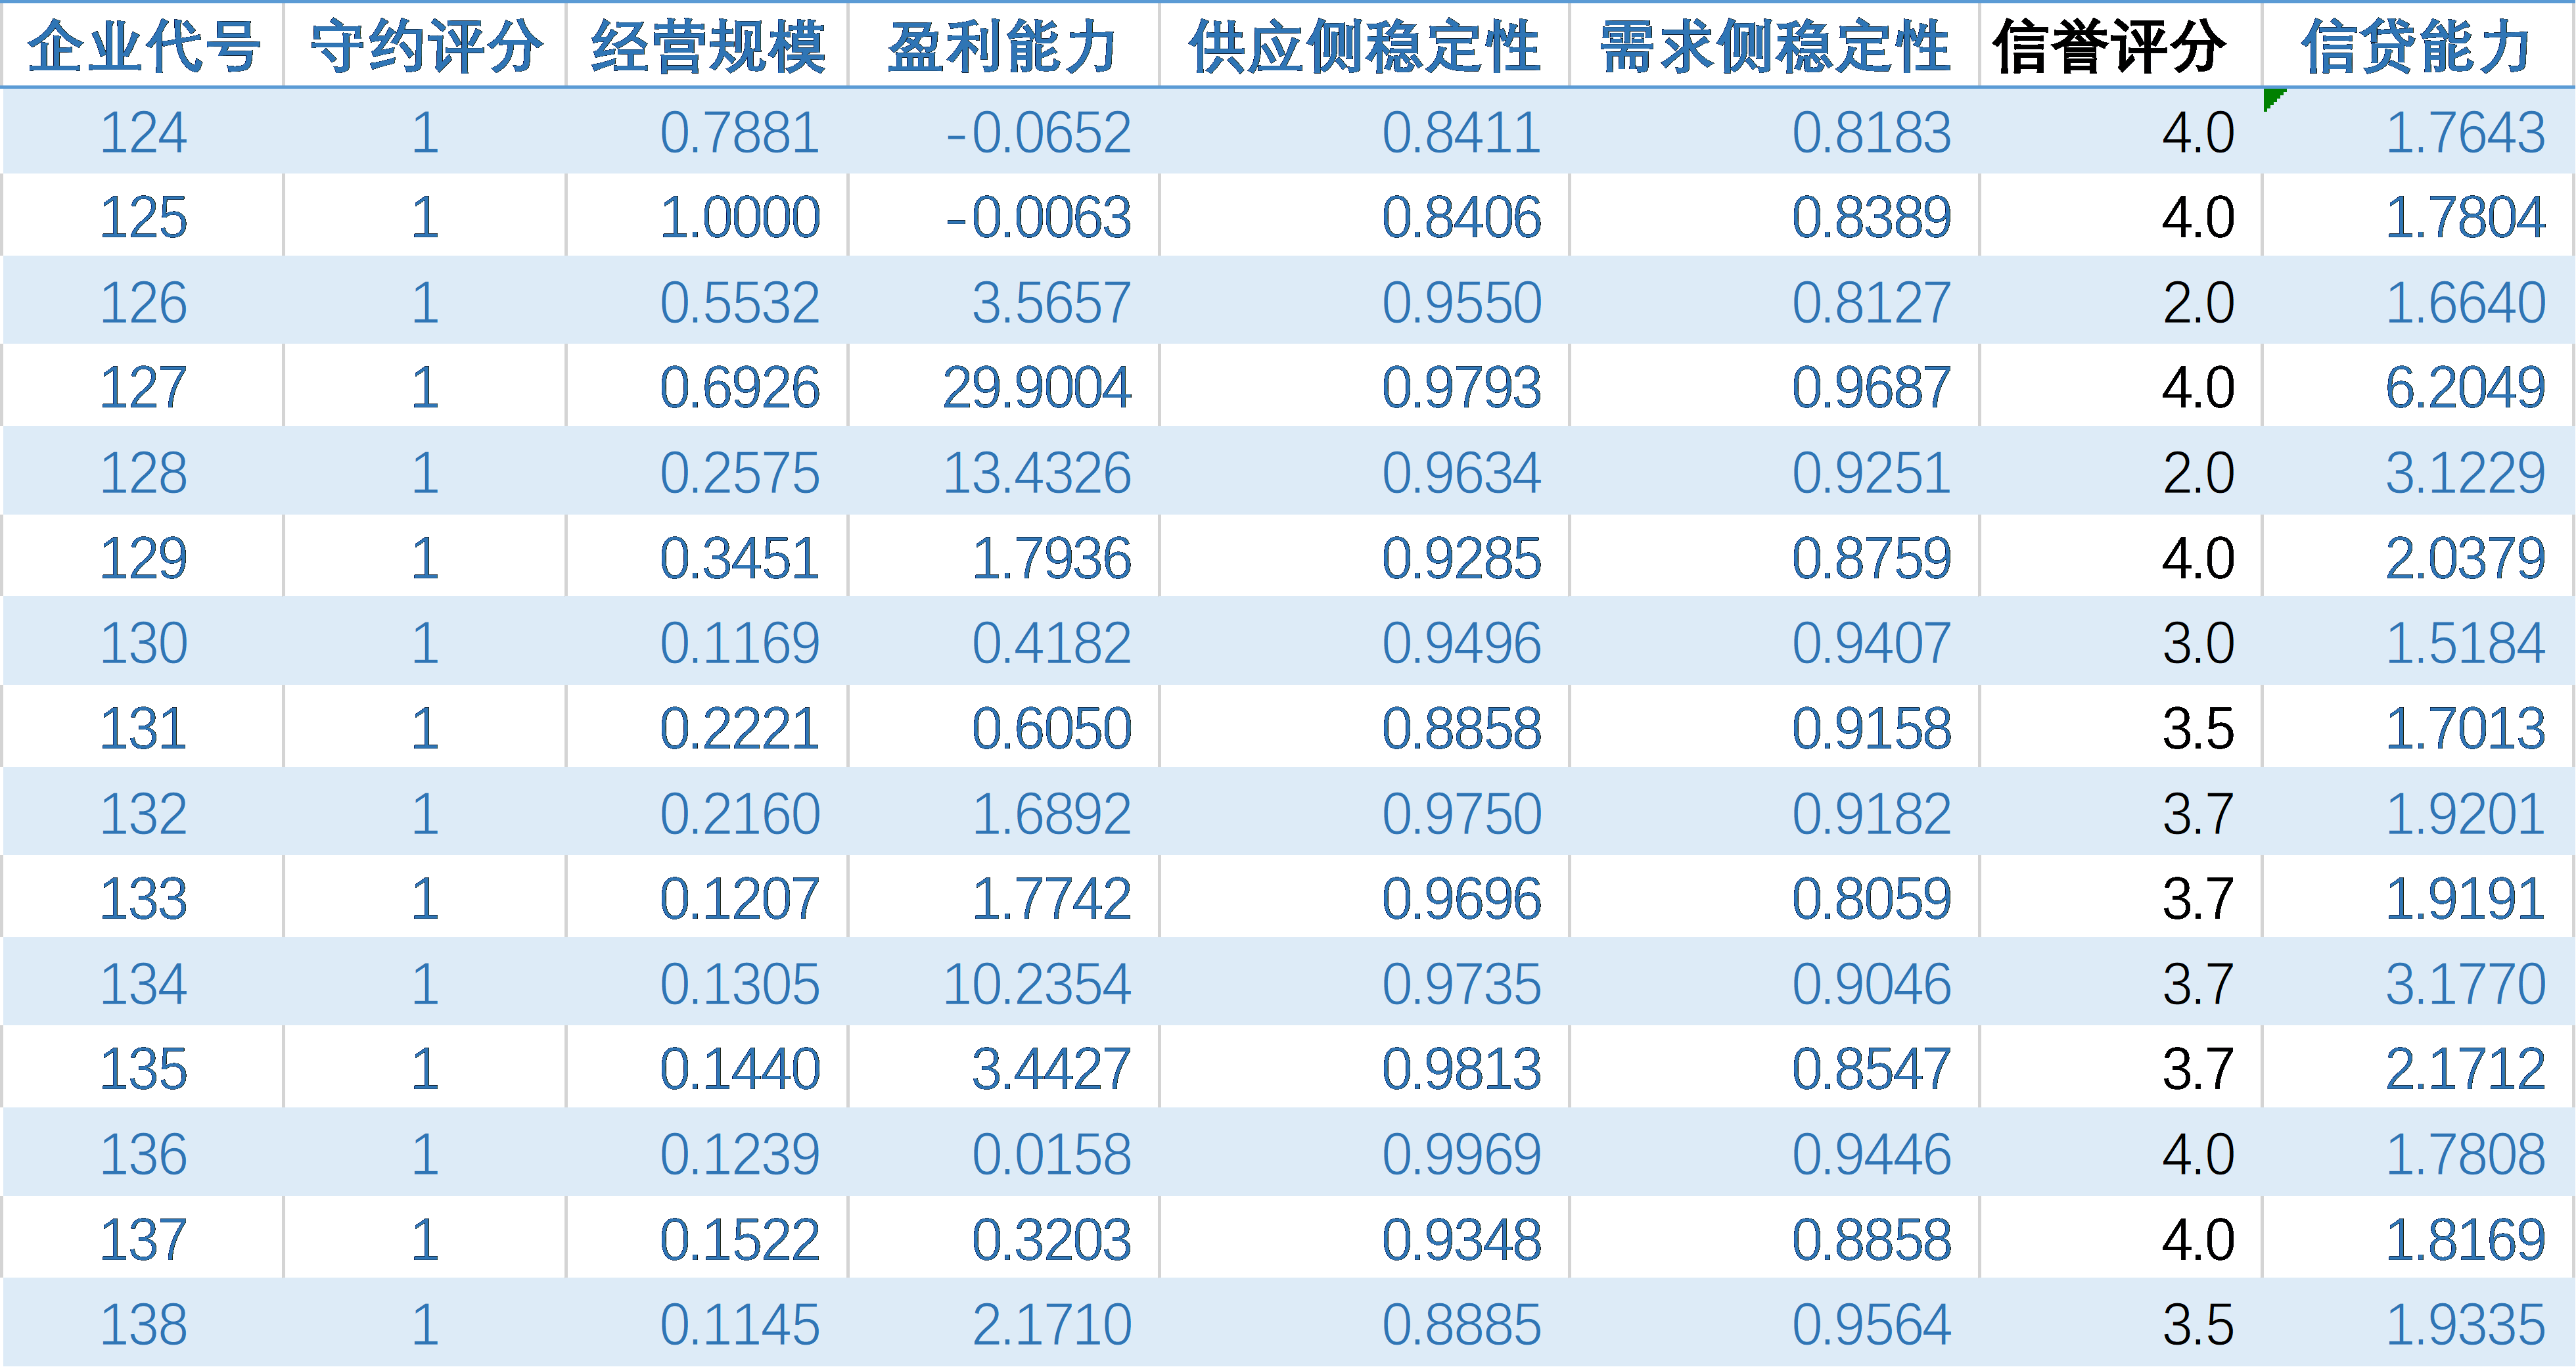
\includegraphics[width=0.75\linewidth]{figure/q2PredictData}%宽度，源文件相对位置
	\caption{部分企业的信贷能力}%图片下方的标题
	\label{fig:q2PredictData}%图片引用时所需标签
\end{figure}

\subsection{规划求解信贷策略}
\subsubsection{规划模型的求解}
在银行年度信贷总额为1亿的约束条件下，我们根据规划求解理论\cite{ref1}建立的信贷策略模型，使银行收入的数学期望值达到最高，即可给出该银行在年度信贷总额为1亿时对这些企业的信贷策略。这里的银行收入的数学期望值就是我们的目标函数。

具体方法同问题一的规划求解方法。首先，在年利率和贷款额度约束条件下，我们结合企业的排位百分比，区分银行是否发放贷款，并将可以贷款的企业的贷款额度和贷款年利率分为与问题一相同的31种档位。接着，我们借助在MATLAB中预先编写好的代码，导入计算出的企业相关数据，并调用函数\verb|linprog()|，具体代码可在附录中查看，得出302家企业实际贷款额度，制定出在银行年度信贷总额为1亿的情况下最为理想的信贷策略。具体结果策略如下图所示。所得银行收入的数学期望值$5.0157 \times {10^4}$。

\begin{figure}[H]
	\centering
	
\includegraphics[width=0.75\linewidth]{figure/q2ResultTable}%宽度，源文件相对位置
	\caption{规划求解所得的信贷策略}%图片下方的标题
	\label{fig:q2ResultTable}%图片引用时所需标签
\end{figure}







%分文件结束
\ifx\allfiles\undefined
\end{document}
\fi